\documentclass[letterpaper]{article} % DO NOT CHANGE THIS
\usepackage[submission]{aaai24}  % DO NOT CHANGE THIS
\usepackage{times}  % DO NOT CHANGE THIS
\usepackage{helvet}  % DO NOT CHANGE THIS
\usepackage{courier}  % DO NOT CHANGE THIS
\usepackage[hyphens]{url}  % DO NOT CHANGE THIS
\usepackage{graphicx} % DO NOT CHANGE THIS
\urlstyle{rm} % DO NOT CHANGE THIS
\def\UrlFont{\rm}  % DO NOT CHANGE THIS
\usepackage{natbib}  % DO NOT CHANGE THIS AND DO NOT ADD ANY OPTIONS TO IT
\usepackage{caption} % DO NOT CHANGE THIS AND DO NOT ADD ANY OPTIONS TO IT
\frenchspacing  % DO NOT CHANGE THIS
\setlength{\pdfpagewidth}{8.5in} % DO NOT CHANGE THIS
\setlength{\pdfpageheight}{11in} % DO NOT CHANGE THIS
%
% These are recommended to typeset algorithms but not required. See the subsubsection on algorithms. Remove them if you don't have algorithms in your paper.
\usepackage{algorithm}
\usepackage{algorithmic}

%
% These are are recommended to typeset listings but not required. See the subsubsection on listing. Remove this block if you don't have listings in your paper.
\usepackage{newfloat}
\usepackage{listings}

% User imported packages
\usepackage{multirow}
\usepackage{pifont}
\usepackage{booktabs}
\usepackage{subcaption}
\usepackage{bm}
\usepackage{amsmath}
\usepackage{amssymb}
\usepackage{cleveref}
\usepackage{todonotes}
\usepackage{varwidth}
\usepackage{tikz}
\usepackage{graphicx}
\newcommand{\cmark}{\ding{51}} % checkmark symbol
\newcommand{\xmark}{\ding{55}} % X-mark symbol

\DeclareCaptionStyle{ruled}{labelfont=normalfont,labelsep=colon,strut=off} % DO NOT CHANGE THIS
\lstset{%
	basicstyle={\footnotesize\ttfamily},% footnotesize acceptable for monospace
	numbers=left,numberstyle=\footnotesize,xleftmargin=2em,% show line numbers, remove this entire line if you don't want the numbers.
	aboveskip=0pt,belowskip=0pt,%
	showstringspaces=false,tabsize=2,breaklines=true}
\floatstyle{ruled}
\newfloat{listing}{tb}{lst}{}
\floatname{listing}{Listing}
%
% Keep the \pdfinfo as shown here. There's no need
% for you to add the /Title and /Author tags.
\pdfinfo{
/TemplateVersion (2024.1)
}

% DISALLOWED PACKAGES
% \usepackage{authblk} -- This package is specifically forbidden
% \usepackage{balance} -- This package is specifically forbidden
% \usepackage{color (if used in text)
% \usepackage{CJK} -- This package is specifically forbidden
% \usepackage{float} -- This package is specifically forbidden
% \usepackage{flushend} -- This package is specifically forbidden
% \usepackage{fontenc} -- This package is specifically forbidden
% \usepackage{fullpage} -- This package is specifically forbidden
% \usepackage{geometry} -- This package is specifically forbidden
% \usepackage{grffile} -- This package is specifically forbidden
% \usepackage{hyperref} -- This package is specifically forbidden
% \usepackage{navigator} -- This package is specifically forbidden
% (or any other package that embeds links such as navigator or hyperref)
% \indentfirst} -- This package is specifically forbidden
% \layout} -- This package is specifically forbidden
% \multicol} -- This package is specifically forbidden
% \nameref} -- This package is specifically forbidden
% \usepackage{savetrees} -- This package is specifically forbidden
% \usepackage{setspace} -- This package is specifically forbidden
% \usepackage{stfloats} -- This package is specifically forbidden
% \usepackage{tabu} -- This package is specifically forbidden
% \usepackage{titlesec} -- This package is specifically forbidden
% \usepackage{tocbibind} -- This package is specifically forbidden
% \usepackage{ulem} -- This package is specifically forbidden
% \usepackage{wrapfig} -- This package is specifically forbidden
% DISALLOWED COMMANDS
% \nocopyright -- Your paper will not be published if you use this command
% \addtolength -- This command may not be used
% \balance -- This command may not be used
% \baselinestretch -- Your paper will not be published if you use this command
% \clearpage -- No page breaks of any kind may be used for the final version of your paper
% \columnsep -- This command may not be used
% \newpage -- No page breaks of any kind may be used for the final version of your paper
% \pagebreak -- No page breaks of any kind may be used for the final version of your paperr
% \pagestyle -- This command may not be used
% \tiny -- This is not an acceptable font size.
% \vspace{- -- No negative value may be used in proximity of a caption, figure, table, section, subsection, subsubsection, or reference
% \vskip{- -- No negative value may be used to alter spacing above or below a caption, figure, table, section, subsection, subsubsection, or reference

\setcounter{secnumdepth}{0} %May be changed to 1 or 2 if section numbers are desired.

% The file aaai24.sty is the style file for AAAI Press
% proceedings, working notes, and technical reports.
%

% Title

% Your title must be in mixed case, not sentence case.
% That means all verbs (including short verbs like be, is, using,and go),
% nouns, adverbs, adjectives should be capitalized, including both words in hyphenated terms, while
% articles, conjunctions, and prepositions are lower case unless they
% directly follow a colon or long dash
\iffalse\title{AAAI Press Anonymous Submission\\Instructions for Authors Using \LaTeX{}}
\author{
    %Authors
    % All authors must be in the same font size and format.
    Written by AAAI Press Staff\textsuperscript{\rm 1}\thanks{With help from the AAAI Publications Committee.}\\
    AAAI Style Contributions by Pater Patel Schneider,
    Sunil Issar,\\
    J. Scott Penberthy,
    George Ferguson,
    Hans Guesgen,
    Francisco Cruz\equalcontrib,
    Marc Pujol-Gonzalez\equalcontrib}
\affiliations{
    %Afiliations
    \textsuperscript{\rm 1}Association for the Advancement of Artificial Intelligence\\
    % If you have multiple authors and multiple affiliations
    % use superscripts in text and roman font to identify them.
    % For example,

    % Sunil Issar\textsuperscript{\rm 2},
    % J. Scott Penberthy\textsuperscript{\rm 3},
    % George Ferguson\textsuperscript{\rm 4},
    % Hans Guesgen\textsuperscript{\rm 5}
    % Note that the comma should be placed after the superscript

    1900 Embarcadero Road, Suite 101\\
    Palo Alto, California 94303-3310 USA\\
    % email address must be in roman text type, not monospace or sans serif
    proceedings-questions@aaai.org
%
% See more examples next
}
\fi

%Example, Single Author, ->> remove \iffalse,\fi and place them surrounding AAAI title to use it
\iffalse\title{My Publication Title --- Single Author}
\author{
    Author Name
}
\affiliations{
    Affiliation\\
    Affiliation Line 2\\
    name@example.com
}
\fi

%Example, Multiple Authors, ->> remove \iffalse,\fi and place them surrounding AAAI title to use it
\title{The Right Learning Rate at the Right Time}
\author{
    % Authors
    Lucas Cazzonelli\textsuperscript{\rm 1},
    Cedric Kulbach\textsuperscript{\rm 2},
}
\affiliations{
    % Affiliations
    \textsuperscript{\rm 1}FZI Research Center for Information Technology\\
    \textsuperscript{\rm 2}Affiliation 2\\
    cazzonelli@fzi.de, secondAuthor@affilation2.com
}


% REMOVE THIS: bibentry
% This is only needed to show inline citations in the guidelines document. You should not need it and can safely delete it.
\usepackage{bibentry}
% END REMOVE bibentry

\begin{document}

\maketitle


\begin{abstract}

	\noindent The selection of an appropriate optimizer plays a crucial role in deep learning, significantly influencing model performance.
	In the context of batch learning, where all data is available at a time, extensive research has been conducted to understand the implications of different optimizer choices and various optimization techniques for deep learning architectures have emerged.
	However, when it comes to online learning, where models need to adapt to evolving data streams, the exploration of optimizer choices is still relatively limited. \todo{Decide on which term to use. Online Learning vs. Stream Learning etc. Online sounds better but might be confusing since SGD is technically always an online algo.}
	This paper focuses on bridging the gap in knowledge by investigating how the choice of optimizer  changes from batch learning to online learning scenarios.
	Our study conducts an in-depth analysis on the impact of optimizer, learning rate and batch size on the (i) predictive performance as well as the capability of adapting to changes on the underlying data pattern that might occur over time within the evolving data stream.
	Additionally, we explore practical choices for gradient-based online training of deep architectures, with a specific emphasis on adaptive methods.
	These methods dynamically adjust the learning rate based on gradient characteristics, offering potential advantages in online learning scenarios.
	\todo{Add more text.}

\end{abstract}

\section{Introduction}
Deep learning models have demonstrated exceptional performance in various domains, with the choice of optimizer playing a crucial role in achieving outstanding results.
In the context of batch learning, where all data is available simultaneously, extensive research has been conducted to explore different optimizer choices and optimization techniques for deep learning architectures.
Numerous methods have emerged to effectively update the weights of these architectures.
However, the investigation of optimizer choices in online learning, where models must adapt to evolving data streams, remains relatively limited.

This paper aims to bridge this knowledge gap by investigating how the choice of optimizer changes when transitioning from batch learning to online learning scenarios. Specifically, we address the following research questions:
\begin{itemize}
	\item How does the choice for the optimizer change from batch to online learning?
	\item What are practical choices for gradient-based online training of deep architectures in online learning?
	\item Are adaptive optimization methods better suited in Online Deep Learning?
\end{itemize}
\todo{Put LR tuning graphic here?}
\begin{figure}[ht]
	\centering
	\begin{tikzpicture}
		% Upper image
		\node[inner sep=0pt] (upper) {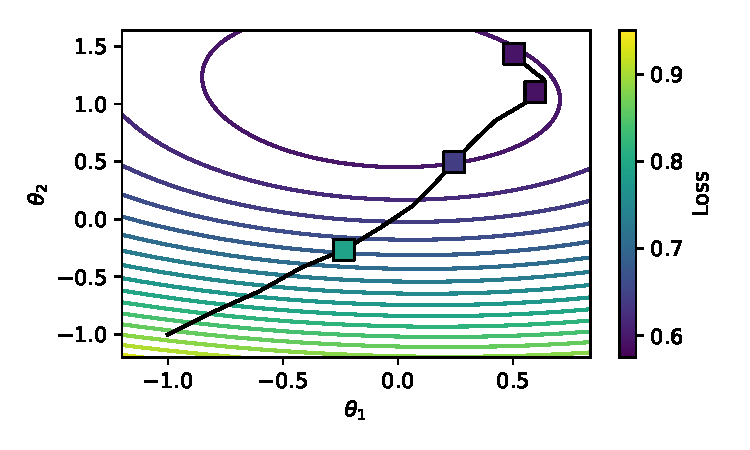
\includegraphics[width=0.4\textwidth]{figures/adam_trajectory_drift_reset1.pdf}};

		% Lower image
		\node[inner sep=0pt, below=3mm of upper] (lower){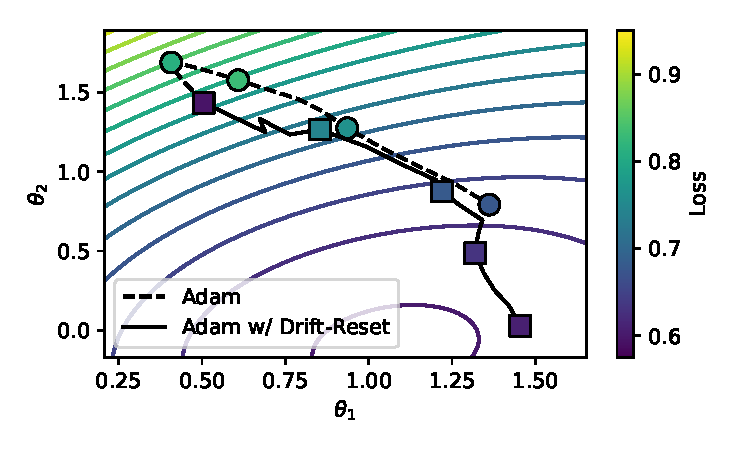
\includegraphics[width=0.4\textwidth]{figures/adam_trajectory_drift_reset2.pdf}};

		\path ([xshift=-8pt]upper) -- ([xshift=-8pt]lower) node[midway] (text){Concept Drift};
		\draw[->] ([xshift=-5pt, yshift=5pt]upper.south-|text.west) -- ([xshift=-5pt, yshift=-3pt]lower.north-|text.west);
		\draw[->] ([xshift=5pt, yshift=5pt]upper.south-|text.east) -- ([xshift=5pt, yshift=-3pt]lower.north-|text.east);

	\end{tikzpicture}
	\caption{Parameter trajectory of Adam~\cite{kingmaAdamMethodStochastic2017b} with or without adaptation to concept drift on synthetic data stream with abrupt concept drift. Marker colors depict the expected prequential loss over the last 16 data instances.}
\end{figure}
For the first research question, we explore how the selection of an optimizer differs when moving from the traditional batch learning setting to the dynamic online learning scenario. We examine the suitability of various optimizer choices in online learning and their impact on model performance.

The second research questions investigates practical choices for gradient-based online training of deep architectures.
We analyze different optimization techniques and explore their effectiveness in adapting to evolving data streams while maintaining model performance.
The third research question focuses on the performance of adaptive methods in online deep learning scenarios.
These methods dynamically adjust the learning rate based on gradient characteristics, allowing models to adapt more effectively to changing data patterns. We compare the performance of adaptive methods against other optimization approaches to determine their suitability for online deep learning tasks.
Through our in-depth analysis and experimentation, we aim to enhance our understanding of optimizer choices in online deep learning.
By shedding light on the impact of optimizers, learning rates, and batch sizes, and comparing the effectiveness of adaptive methods, we aim to enable researchers and practitioners to make informed decisions when selecting optimization techniques for real-time learning tasks.



\subsection{Research Questions}
\begin{itemize}

	\item How does the choice for the optimizer change from batch to online learning?
	      -> Batch learning: goal maximize batch size for best performance -> suitable for online learning?
	      -> Learning Rate
	      -> In-depth analysis on the influence of the learning rate and batch size on the effectiveness of online stochastic gradient descent
	      -> Grafik SGD,
	\item What are practical choices for gradient-based online training of deep architectures in online learning?
	      -> Description adaptive methods
	\item Are adaptive methods better suited in Online Deep Learning?
	      -> Table with results
\end{itemize}

Motivation:
\begin{itemize}
	\item Learning rate is one of the most important hyperparameters when it comes to training deep learning models.
	\item A small learning rate causes slow convergence, while an excessive learning rate causes instability (observable in the form of oscillations) or even increases in the training objective.
	\item \citet{bengioPracticalRecommendationsGradientbased2012} goes as far as to say that out of all possible hyperparameters, if any, the learning rate is the one to be tuned.
	\item This applies arguably even more so to online learning. Unlike in batch learning, for instance, repeating the entire process if training diverges is infeasible, due to the restriction that previously observed data samples can, if at all, only be stored in small numbers.
	\item Furthermore, the trained model must be ready to predict at any given moment meaning that an inadequate learning rate has an immediate impact on the quality of generated predictions.
	\item In batch learning it is still common practice to determine the learning rate by running multiple training runs, beginning with a high learning rate and restarting the process with a lower learning rate every time the objective value diverges~\cite{bengioPracticalRecommendationsGradientbased2012}.
\end{itemize}

Contributions:
\begin{itemize}
	\item In-depth analysis on the influence of the learning rate and batch size on the effectiveness of online stochastic gradient descent
	\item Experimental comparison of different SGD-based optimizers
	\item Investigation into possible approaches for determining an appropriate learning rate
\end{itemize}

\section{Learning Rate Scheduling}

In the following, we will briefly outline the most important differences between the influence of the learning rate of first order gradient-based optimization methods in streaming- and in conventional batch learning environments.

First order gradient-based optimization approaches like stochastic gradient descent and its derivatives aim to iteratively minimize the error of a DL model using only first order gradient information at each step $t$. We denote the gradient of the prediction error for a mini-batch of training samples $y_t, X_t \sim p_t$ with respect to model-parameters $\theta$ as
\begin{equation}
	g_t(\theta)   =   \nabla_{\theta} \mathcal{L}(y_t, f(X_t; \theta)),
\end{equation}
where $\mathcal{L}$ represents a loss function (e.g., cross-entropy for classification- or mean squared error for regression tasks). Using this notation, the update performed by SGD with a constant learning rate $\eta$ at each iteration $t$ is given by
\begin{equation}
	\theta_{t+1}  = \theta_{t} - \eta \cdot g_t(\theta_t).
\end{equation}

Many previous works deal with the intricacies of SGD in the context of training deep architectures in a batch learning setting (see \citet{bengioPracticalRecommendationsGradientbased2012,bottouStochasticGradientDescent2012,Goodfellow-et-al-2016}).
The primary trade-off identified by these works when it comes to  the selection of an appropriate learning rate is that between the speed of convergence and the amount of stochasticity.
While increasing the learning rate speeds up convergence, it also increases stochasticity and therefore leads to the divergence of the training criterion beyond a certain threshold.
\Citet{smithBayesianPerspectiveGeneralization2018} for instance, found that when modelling SGD as a stochastic differential equation, the “noise scale” is directly tied to $\eta$~\cite{smithBayesianPerspectiveGeneralization2018}.
In biological terms, increasing the learning rate increases plasticity, whereas decreasing it increases stability. % Maybe remove? I like the biological analogy, but there are no sources supporting the claim. 


To get the best out of large and small values for $\eta$, a learning rate schedule $(\eta_1,\ldots,\eta_T)$, which assigns a learning rate to each update step $t \in 1,\ldots,T$ can be used.
It is for instance common to set a high learning rate initially and decrease it throughout the training process.
This ensures fast convergence and a higher level of noise at the start of training, which has been claimed to help SGD skip over sharp minima with poor generalization~\cite{hochreiterFlatMinima1997,chaudhariEntropySGDBiasingGradient2017}, while mitigating jumping around potential minima at later stages.
Some have likened this procedure to simulated annealing, which shifts its focus from exploration at high temperatures to exploitation once temperatures have sufficiently decreased~\cite{smithDonDecayLearning2018}.

A simple way to achieve such a schedule is to exponentially decay $\eta$ after each update by multiplying it with a factor $\gamma < 1$, although some practitioners have come to prefer schedules with sharper drop-offs like step schedules that decrease $\eta$ by a larger margin after a certain number of updates~\cite{smithDonDecayLearning2018}.
Other popular options include cyclic learning rate schedules which oscillate  $\eta$ between a base- and a maximum or minimum value over a predefined interval.
Some studies~\cite{smithCyclicalLearningRates2017, smithSuperConvergenceVeryFast2018a} have found cyclic schedules to significantly speed up the convergence of neural networks even when compared to adaptive techniques like Adam~\cite{kingmaAdamMethodStochastic2017b}.
\Citet{wuDemystifyingLearningRate2019b} provide a detailed analysis on the effect of learning rate policies like the aforementioned ones.

In contrast to the field of conventional batch learning, the impact of the learning rate in stream-based deep learning is a lesser studied issue. According to \citet{bifetMOAMassiveOnline2010} a machine learning model operating in such an environment must be able to
\begin{center}
	\begin{varwidth}{0.5\textwidth}
		\begin{description}
			\item[R1:] process a single instance at a time,\label{rq:single_instance}
			\item[R2:] process each instance in a limited amount of time,\label{rq:limited_time}
			\item[R3:] use a limited amount of memory,\label{rq:limited_memory}
			\item[R4:] predict at any time,\label{rq:predict_any_time}
			\item[R5:] adapt to changes in the data distribution.\label{rq:adapt_to_drift}
		\end{description}
	\end{varwidth}
\end{center}
These requirements lead to significant differences with respect to the problem of learning rate optimization compared to batch learning.
Nevertheless, only few studies on the impact and tuning of the learning rate in stream-based deep learning exist.


In batch learning, the task of finding an optimal schedule for $\eta$ can be defined as
\begin{equation}
	\label{eq:batch_lr_optim}
	\begin{alignedat}{3}
		& \!\min_{\eta_0, \ldots, \eta_T} & \, & \sum_{i=1}^{V}\mathcal{L}(y_i, f(X_i; \theta_T)) &    &                              \\
		& \text{s.t.}                     &    & X_i, y_i  \sim p^{(v)}                           & \  & \forall i \in {1, \ldots, V}
		,
	\end{alignedat}
\end{equation}
where $p^{(v)}$ is a distribution of validation data, usually made up of a dataset split off from the training dataset.
Verbally, learning rate optimization in batch learning aims to find a schedule $(\eta_0, \ldots, \eta_T)$ leading to parameter values $\theta_T$ at the end of a training run that in turn minimize the prediction error for validation data.

Under the requirements described above, however, we must define the task differently as
\begin{equation}
	\label{eq:stream_lr_optim}
	\begin{alignedat}{3}
		& \!\min_{\eta_0, \ldots, \eta_T} & \, & \sum_{t=0}^{T}\mathcal{L}(y_t, f(X_t; \theta_{t-1})) &    &                               \\
		& \text{s.t.}                     &    & X_t, y_t  \sim p_t                           & \  & \forall t \in {1, \ldots, T}.
	\end{alignedat}
\end{equation}
Compared to Problem~\eqref{eq:batch_lr_optim}, the most apparent difference is that there is no separate validation data.
Instead, due to Requirement~\ref{rq:predict_any_time}, the goal is to minimize $\mathcal{L}$ with respect to the next instances $X_{t+1}, y_{t+1}$ at each timestep $t$.

This means that in contrast to Problem~\eqref{eq:batch_lr_optim}, not only the final parameters $\theta_T$ but every parameter configuration $\theta_t$ in the entire trajectory contributes equally to the objective.
Therefore, speed of convergence is of much larger importance in the streaming setting, whereas the performance of the final parameters $\theta_T$ has relatively little impact.
Since memory is limited (Requirement~\ref{rq:limited_memory}), it is also not possible to continue training on previously observed data as long as $\mathcal{L}$ decreases, which puts an even greater emphasis on quick adaptation.
At the same time, a larger learning rate causing temporary loss increases, due to skipping over sharp minima can be suboptimal with respect to Problem~\ref{eq:stream_lr_optim} even if it eventually yields a lower loss.
Another difference to conventional batch learning is that the distribution $p_t$ of the data stream might, and in practice most likely will, be subjected to change in the form of concept drift over time.
Under such circumstances, the optimal parameter values $\theta^*$ move throughout the progression of the stream increasing the distance to the model parameters.

Since the theoretically optimal learning rate $\eta^*$ is proportional to the quadratic distance between initial and optimal parameters $||\theta_1 - \theta^*||^2$ (albeit under some constraints like the absence of noise)~\cite{carmonMakingSGDParameterFree2023}, it should be larger when concept drift occurs.

Based on this notion, \citet{kunchevaAdaptiveLearningRate2008} introduced an adaptive schedule that updates the learning rate using
\begin{equation}
	\eta_{t+1} = \eta_t^{1+(\mathcal{L}_t - \bar{\mathcal{L}}_{t-1})},
\end{equation}
where $\mathcal{L}_t$ represents the loss for the current sample, and $\bar{\mathcal{L}}_{t-1}$ a rolling mean of past losses.
By doing so, \citet{kunchevaAdaptiveLearningRate2008} increases in loss lead to increases in the learning rate and vice versa.
While this approach seems intuitively sound, it bears a high risk of $\eta$ increasing indefinitely, since increases in loss caused by an excessive learning rate would lead to a feedback loop.

We therefore propose a simple adaptation to popular decaying learning rate schedules that operates in a fixed value range and increases the model's plasticity when needed by resetting $\eta$ to its original value if a concept drift has occurred.
To this end we apply an ADWIN drift detector~\cite{bifetLearningTimeChangingData2007} to the underlying model's prequential loss to reduce the drift detection task to a computationally less expensive univariate problem.
While our approach does not allow for a continuous adaptation like the technique by \citet{kunchevaAdaptiveLearningRate2008} and might therefore be less suited for more subtle drift, it offers more reliability since the initial learning rate cannot be exceeded.
\todo{Talk about drift-probability dependent resetting with P-KSWIN?}

Concept drift also complicates the tuning of $\eta$, since even if data is available beforehand drift would eventually cause the stream to diverge from the distribution of data used for tuning.
% In our experiments we investigate to which extent this effect impairs learning rate tuning on data available prior to deployment of a stream-based neural net. 
This effect, combined with the previously described differences in the evaluation scheme can cause conventional learning rate tuning to produce unsuitable results for stream-based learning.
% Alternatively: 
% Furthermore, in conventional batch learning, the standard practice for learning rate tuning is to optimize for the performance on the validation data~\cite{defazioLearningRateFreeLearningDAdaptation2023a}.
% As a result, this approach disregards the performance of the model throughout the tuning process and only selects the learning rate with the best final performance potentially yielding a value unsuitable for stream-based learning.
We therefore propose a slightly different online learning specific tuning approach, that aims to approximately solve Problem~\ref{eq:stream_lr_optim}.

To emulate
% a static version of 
the targeted data stream we continually draw samples with replacement from the tuning data in a bootstrapping procedure instead of training on all data for multiple epochs.
By doing so we aim to increase data variability% better: randomness?
, and therefore the resemblance to an actual data stream with random distributional shifts.
We then optimize $\eta$ with respect to the mean prequential performance over the emulated stream instead of the performance on a validation set.
For this purpose we use a basic grid-search as is customary in batch learning~\cite{defazioLearningRateFreeLearningDAdaptation2023a}.
We provide a detailed experimental evaluation of our approach in Section~\ref{sec:experiments}.


\section{Parameter-Free Optimizers}

While determining the learning rate through a separate tuning phase with parameter searches like grid- or random-search is still the de facto standard in deep learning~\cite{defazioLearningRateFreeLearningDAdaptation2023a}, this approach causes significant computational overhead.
To avoid this overhead, several previous works have developed parameter-free variants of SGD (see Table~\ref{tab:param_free_optims}) that estimate the optimal step size online as training progresses, eliminating the learning rate entirely.

In one of the earlier works, \citet{schaulNoMorePesky2013} proposed \textit{vSGD}, which uses first and second order moments of the gradients as well as local curvature information~\cite{schaulNoMorePesky2013} to estimate $\eta$.
The authors obtain the latter by estimating positive diagonal entries of the Hessian with respect to the parameters through a back-propagation formula~\cite{schaulNoMorePesky2013}.
Even though \citet{schaulNoMorePesky2013} demonstrate \textit{vSGD's} robustness to non-stationary data distributions, it has, to the best of our knowledge, not been widely adopted in the online learning space. \todo{Did not evaluate vSGD since its old and there is no implementation yet. Is that valid?}

Instead of using curvature information for adapting $\eta$, the \textit{COCOB} optimizer proposed by \citet{orabonaTrainingDeepNetworks2017} 


Furthermore, several studies developed paramater-free optimizers for specific areas of application such as time series forecasting~\cite{miyaguchiCograConceptDriftAwareStochastic2019,fekriDeepLearningLoad2021, zhangPOLAOnlineTime2021a}, federated learning~\cite{canonacoAdaptiveFederatedLearning2021} and recommender systems~\cite{ferreirajoseADADRIFTAdaptiveLearning2020}.
Due to our focus for the present work being general data stream applications, we did not further investigate these techniques either.

Besides \citet{schaulNoMorePesky2013} none of these optimizers target batch learning scenarios and therefore do not explicitly consider concept drift, which raises the question of whether they are suitable for stream-based learning.
Previous work on parameter-free optimization of online deep learning models is rather limited, and mostly focused on specific applications.

\begin{table}[]
	\centering
	\begin{tabular}{@{}lllc@{}}
		\toprule
		Optimizer & Complexity                      & Space             & Param. specific \\ \midrule
		DAdapt    & $\mathcal{O}(6D)$               & $\mathcal{O}(2D)$ & \xmark          \\
		DoG       & $\mathcal{O}(5D)$               & $\mathcal{O}(1D)$ & \xmark          \\
		Mechanic  & $\mathcal{O}(4D)$               & $\mathcal{O}(1D)$ & \xmark          \\
		WNGrad    & $\mathcal{O}(2D)$               & $\mathcal{O}(0)$  & \xmark          \\
		SGDHD     & $\mathcal{O}{4D}$               & $mathcal{O}{}$    & \xmark          \\
		COCOB     & $\mathcal{O}(14D)$              & $\mathcal{O}(4D)$ & \cmark          \\
		vSGD      & $\mathcal{O}(21D)$\footnotemark & $\mathcal{O}(4D)$ & \cmark          \\
		\bottomrule
	\end{tabular}
	\caption{Overview of additional time- and space-complexity of parameter-free first-order optimizers compared to basic SGD. Values are given in big O notation with respect to the number of model parameters $D$.}\label{tab:param_free_optims}
\end{table}
\footnotetext[1]{Complexity for feed-forward neural networks. Since \textit{vSGD} requires additional backpropagation steps, its complexity is architecture dependent.}

\section{Adaptive Optimizers}\label{sec:adaptive_optims}

In the case of adaptive approaches like SGD with momentum~\cite{rumelhartLearningRepresentationsBackpropagating1986a}, AdaGrad~\cite{duchiAdaptiveSubgradientMethods2011} or Adam~\cite{kingmaAdamMethodStochastic2017b} the learning rate also varies with respect to individual model parameters, in which case
\begin{equation}
	\eta_t \in \mathbb{R}^{D} \qquad \forall t \in 0,\ldots,T.
\end{equation}
For SGD with momentum,
\begin{equation}
	\eta_t = \alpha \cdot \sum_{i=1}^{t} \beta^{t-i} \cdot \frac{g_i}{g_t}
\end{equation}

- Adaptive learning rate optimizers for batch learning \citep{kingmaAdamMethodStochastic2017b,zeilerADADELTAAdaptiveLearning2012a,duchiAdaptiveSubgradientMethods2011,tielemanLecture5rmspropDivide2012}
- Learning-Rate free optimizers \citep{wuWNGradLearnLearning2020,schaulNoMorePesky2013,orabonaTrainingDeepNetworks2017,miyaguchiCograConceptDriftAwareStochastic2019,
	vanervenMetaGradMultipleLearning2016a,baydinOnlineLearningRate2018}



\section{Experiments}\label{sec:experiments}

\begin{table}[ht]
	\small
	\begin{tabular}{@{}clcccc@{}}
		\toprule
		Type                    & Data Stream            & Samples & Features & Classes \\
		\midrule
		\multirow{2}{*}{Synth.} & RBF abrupt             & 20000   & 20       & 5       \\
		                        & RBF incremental        & 20000   & 20       & 5       \\
		\midrule
		\multirow{5}{*}{Real}   & Insects abrupt         & 52848   & 33       & 6       \\
		                        & Insects incremental    & 57018   & 33       & 6       \\
		                        & Insects incr.-grad.    & 24150   & 33       & 6       \\
		                        & Covertype\footnotemark & 100000  & 54       & 7       \\
		                        & Electricity            & 45312   & 8        & 2       \\
		\bottomrule
	\end{tabular}\label{tab:datasets}
	\caption{Datasets used for experimental evaluations.}
\end{table}

\footnotetext[2]{We used the first 100k from a total of 581k examples only.}
% \section{Results}


% \begin{table*}[t]
%     \centering
%     \small
%     \begin{tabular}{lllllll}
%         \toprule
%         Optimizer                & Schedule     & RBF abrupt                     & RBF incr.                      & Covertype                      & Insects abrupt                 & Electricity                    \\
%         \midrule
%         \multirow[c]{7}{*}{SGD}  & Fixed        & 94.79±.32                      & 70.95±2.89                     & 83.42±.50                      & 71.50±.08                      & 73.77±.40                      \\
%                                  & Exp.         & \underline{94.86±.36}          & 72.79±2.35                     & \underline{83.56±.38}          & 71.87±.38                      & 73.90±.55                      \\
%                                  & Exp. Reset   & \underline{94.86±.20}          & 73.77±.98                      & 83.28±.43                      & 71.75±.22                      & 73.85±.64                      \\
%                                  & Step         & \underline{94.94±.24}          & 72.51±1.70                     & \bfseries\underline{83.61±.18} & 71.96±.20                      & 73.57±.89                      \\
%                                  & Step Reset   & \bfseries\underline{94.99±.17} & 72.41±1.75                     & \underline{83.47±.38}          & 71.62±.18                      & 73.70±.88                      \\
%                                  & Cyclic       & 94.79±.32                      & \bfseries\underline{74.96±.86} & \underline{83.44±.08}          & 71.74±.39                      & 68.38±.81                      \\
%                                  & Cyclic Reset & 94.79±.32                      & \underline{74.45±1.69}         & 83.42±.50                      & 71.69±.25                      & 68.52±1.02                     \\ \midrule
%         \multirow[c]{3}{*}{Adam} & Fixed        & 93.45±.30                      & 69.26±5.14                     & 79.01±.27                      & 75.38±.24                      & 69.79±.54                      \\
%                                  & Exp.         & 92.93±.63                      & 64.72±5.35                     & 79.04±.53                      & \bfseries\underline{75.61±.08} & 69.85±.46                      \\
%                                  & Exp. Reset   & 94.03±.48                      & 63.94±2.05                     & 77.27±.48                      & 72.65±.84                      & 69.12±.94                      \\
%         \midrule
%         AdaGrad                  & Fixed        & 92.45±1.37                     & 52.87±6.62                     & 81.68±.35                      & 74.87±.40                      & 76.99±1.20                     \\
%         SGDHD                    & Fixed        & 93.92±.31                      & 72.29±2.90                     & 83.36±.25                      & 70.67±.06                      & 73.83±.32                      \\
%         COCOB                    & Fixed        & 93.40±.38                      & 63.52±2.70                     & 82.27±.46                      & 74.75±.11                      & \bfseries\underline{84.30±.56} \\
%         WNGrad                   & Fixed        & 87.30±.68                      & 44.92±.73                      & 76.98±.15                      & 66.25±.19                      & 70.80±.59                      \\
%         DAdaptSGD                & Fixed        & 74.91±4.22                     & 45.47±2.75                     & 76.69±.79                      & 50.05±11.26                    & 66.03±1.75                     \\
%         DoG                      & Fixed        & 92.73±.59                      & 73.17±2.72                     & 83.07±.64                      & 70.59±.26                      & 71.53±.70                      \\
%         \bottomrule
%     \end{tabular}
%     \caption{Average prequential accuracy [\%] for best learning rate $\eta^*$.}\label{tab:top1_accuray}
% \end{table*}

\begin{table*}[t]
	\centering
	\small
	\begin{tabular}{lllllll}
		\toprule
		Optimizer                & Schedule     & RBF abrupt            & RBF incr.              & Covertype             & Insects abrupt       & Electricity          \\
		\midrule
		\multirow[c]{7}{*}{SGD}  & Fixed        & 93.70±.90             & 69.33±1.36             & 83.08±.18             & 71.12±.08            & 73.12±.42            \\
		                         & Exp.         & 94.00±.52             & 69.24±1.06             & 82.65±.19             & 71.32±.19            & 73.06±.42            \\
		                         & Exp. Reset   & 94.28±.37             & 69.76±.92              & 82.70±.27             & 71.27±.14            & 73.05±.45            \\
		                         & Step         & 94.00±.68             & 69.16±.99              & 82.74±.10             & 71.39±.17            & 72.96±.48            \\
		                         & Step Reset   & 94.04±.70             & 69.75±.81              & 83.03±.13             & 71.19±.14            & 73.18±.50            \\
		                         & Cyclic       & \underline{94.45±.25} & \underline{73.72±1.16} & \bfseries{83.40±.21}  & 71.41±.20            & 67.80±1.03           \\
		                         & Cyclic Reset & \bfseries{94.50±.21}  & \bfseries{73.78±1.15}  & \underline{83.33±.13} & 71.39±.15            & 67.83±1.00           \\ \midrule
		\multirow[c]{3}{*}{Adam} & Fixed        & 92.77±.41             & 66.46±4.39             & 78.85±.22             & \bfseries{75.08±.13} & 69.23±.41            \\
		                         & Exp.         & 92.17±.82             & 63.91±3.52             & 78.53±.27             & 74.88±.15            & 69.33±.40            \\
		                         & Exp. Reset   & 92.83±1.19            & 62.03±2.59             & 77.05±.08             & 72.04±.49            & 68.31±.40            \\
		\midrule
		AdaGrad                  & Fixed        & 91.34±.83             & 50.39±3.60             & 81.07±.22             & 74.31±.34            & 76.64±1.92           \\
		SGDHD                    & Fixed        & 91.03±.45             & 63.38±1.55             & 82.33±.12             & 67.35±.16            & 73.10±.10            \\
		COCOB                    & Fixed        & 93.40±.38             & 63.52±2.70             & 82.27±.46             & 74.75±.11            & \bfseries{84.30±.56} \\
		WNGrad                   & Fixed        & 87.23±1.24            & 44.79±.76              & 76.95±.15             & 66.14±.15            & 70.74±.59            \\
		DAdaptSGD                & Fixed        & 74.91±4.22            & 45.47±2.75             & 76.69±.79             & 50.05±11.26          & 66.03±1.75           \\
		DoG                      & Fixed        & 92.73±.59             & \underline{73.17±2.72} & 83.07±.64             & 70.59±.26            & 71.53±.70            \\
		\bottomrule
	\end{tabular}
	\caption{Average prequential accuracy [\%] for the three best learning rates.}\label{tab:top3_accuray}
\end{table*}

\begin{table*}
	\small
	\centering
	\begin{tabular}{llllll}
		\toprule
		Resetting Approach & RBF abrupt            & RBF incr.              & Covertype           & Insects abrupt        & Electricity           \\
		\midrule
		ADWIN (Two Tailed) & \bfseries{94.28±.37}  & \underline{69.76±.92}  & 82.70±.27           & \underline{71.27±.14} & \underline{73.05±.45} \\
		ADWIN (One Tailed) & \underline{94.25±.38} & \underline{70.22±2.58} & 82.64±.20           & \underline{71.25±.15} & \underline{73.00±.50} \\
		ADWIN Weight Reset & 71.79±.73             & 65.07±.31              & 82.54±.16           & 50.97±.36             & 70.19±1.00            \\
		KSWIN              & \underline{94.23±.55} & \underline{70.10±1.98} & \bfseries 83.01±.06 & \bfseries 71.38±.16   & \underline{73.13±.31} \\
		P-KSWIN            & 93.86±.48             & \bfseries 70.71±1.38   & \bfseries 83.01±.18 & \underline{71.25±.15} & \bfseries 73.26±.43   \\
		\bottomrule
	\end{tabular}
	\caption{Average prequential accuracy [\%] for the three best learning rates.}
\end{table*}



\begin{figure}
	\centering
	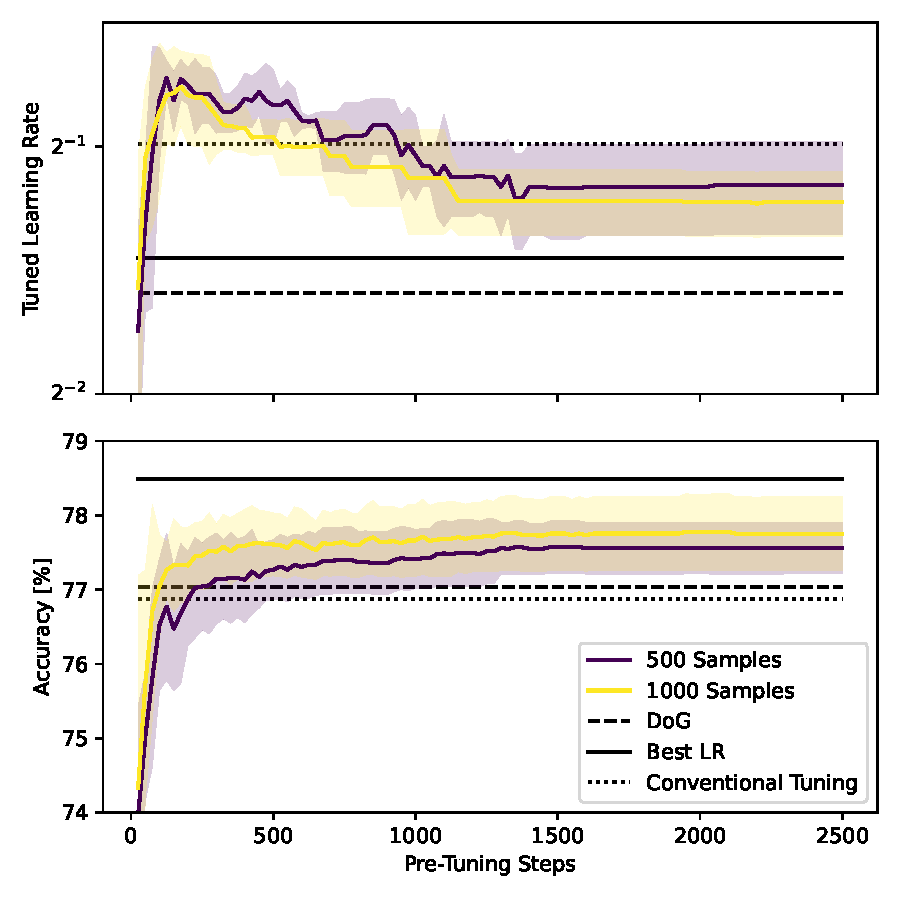
\includegraphics[width=.45\textwidth]{figures/pretune_1x64_acc_lr_exp_schedule.pdf}
	\caption{Pre-tuned LR (LR that maximizes accuracy on pre-tuning data) and resulting accuracy on data streams when using SGD and an exponential learning rate schedule with 500 or 1000 separate tuning samples. Results are averaged over all real-world datasets. The shaded area represents the 1$\sigma$-interval.}\label{fig:pretune_lr_accuracy}
\end{figure}

\begin{figure}
	\centering
	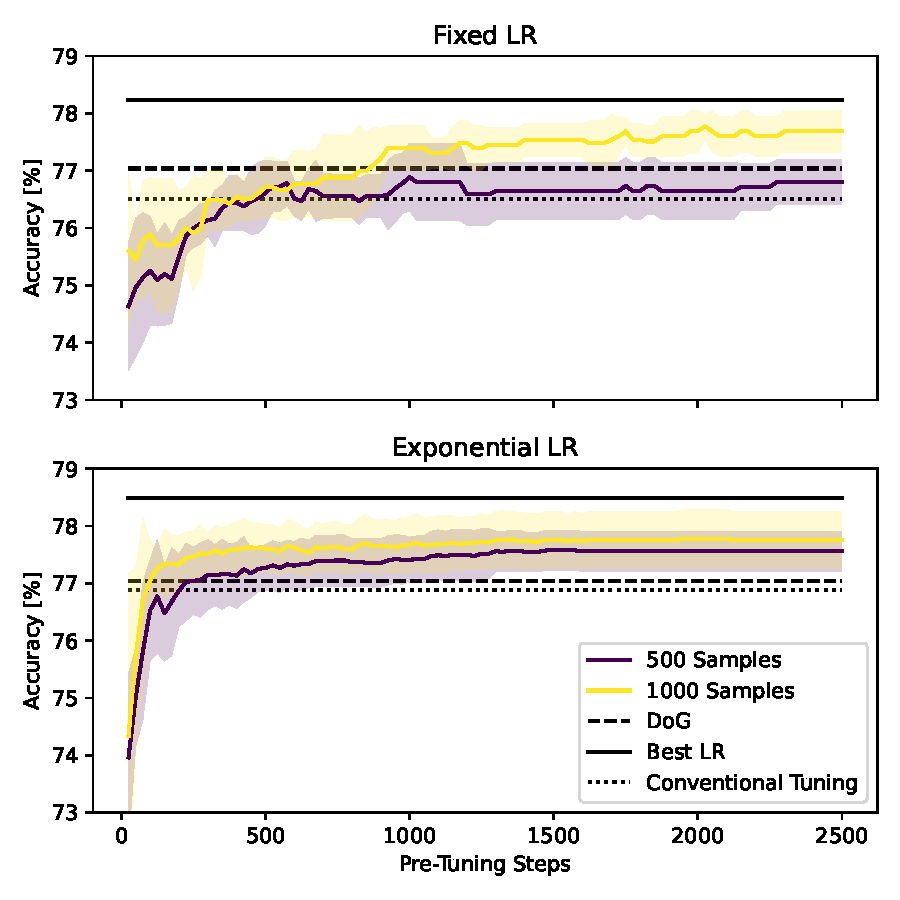
\includegraphics[width=.47\textwidth]{figures/pretune_1x64_fixed_vs_exp_schedule.pdf}
	\caption{Accuracy achieved by pre-tuning on 500 or 1000 samples when using SGD with a fixed LR schedule (top) or an exponential schedule (bottom), averaged over all real-world datasets. The shaded area represents the 1$\sigma$-interval.}\label{fig:pretune_fixed_vs_exp_lr}
\end{figure}

\begin{figure}
	\centering
	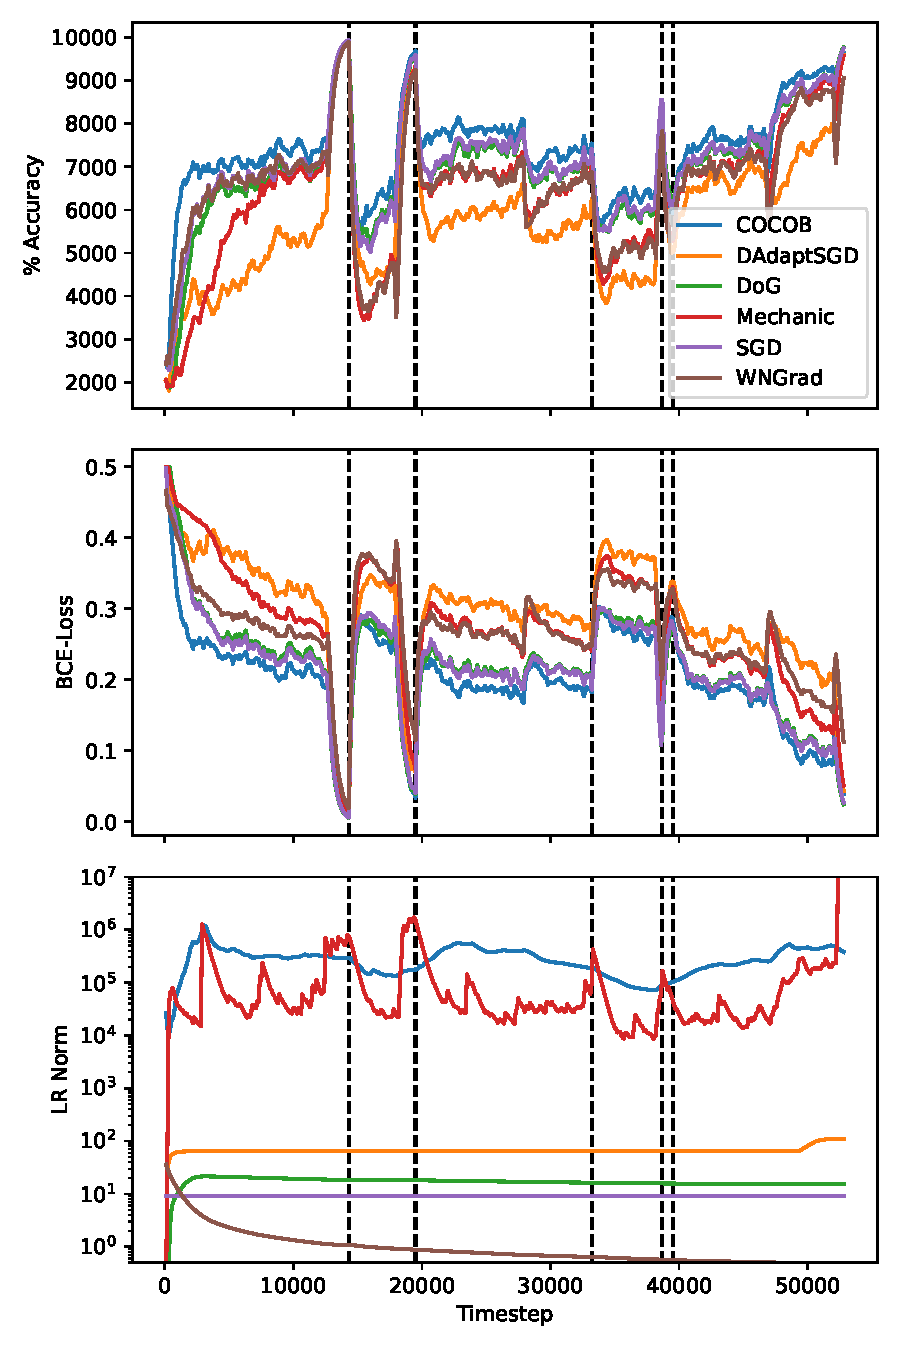
\includegraphics[width=0.47\textwidth]{figures/lr_norms_optims_insects_abrupt.pdf}
	\caption{Prequential accuracy, binary cross-entropy loss and LR norms $||\eta_t||$ over time for various optimization algorithms on Insects abrupt. Each dashed vertical line represents a concept drift. Lines are exponentially smoothed with a factor of 0.8.}
\end{figure}
\begin{figure}
	\centering
	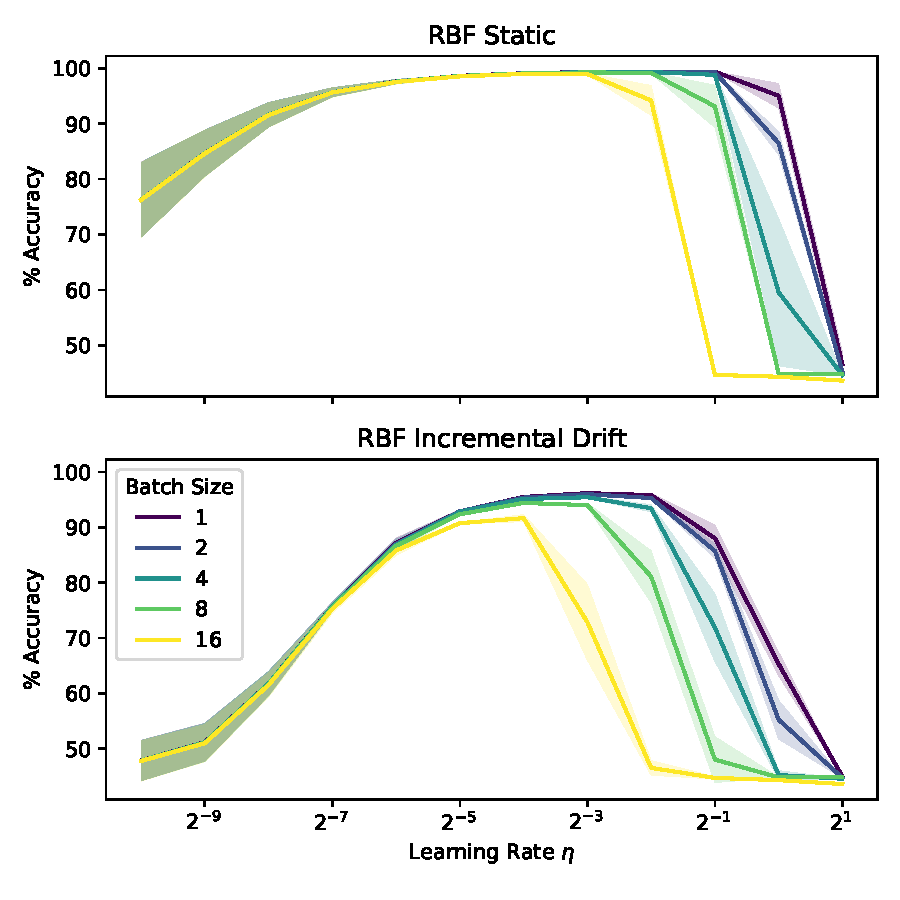
\includegraphics[width=.47\textwidth]{figures/batch_size_lr_wstd.pdf}
	\caption{Average accuracy over static and incrementally drifting synthetic data streams in relation to SGD mini-batch size and learning rate $\eta$. Shaded areas mark the 1$\sigma$ interval.}\label{fig:batch_size_lr}
\end{figure}

\begin{figure}
	\centering
	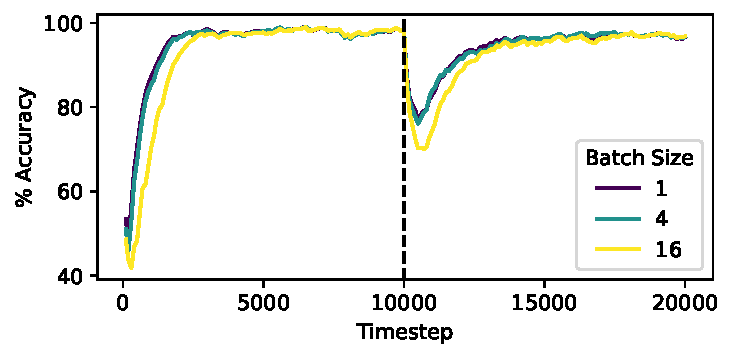
\includegraphics[width=.47\textwidth]{figures/accuracy_vs_time.pdf}
	\caption{Prequential accuracy for different batch sizes on RBF abrupt data stream.}
\end{figure}

We ran prequential evaluations using basic SGD with variable batch sizes and learning rates for synthetic data streams with and without incremental concept drift, the results of which are displayed in \Cref{fig:batch_size_lr}. For static data, the average prequential accuracy over the entire stream gradually improves when moving up from an inadequately low learning rate until a certain point where training begins to diverge and performance consequently crashes. Based on our results, there seems to be an inverse relationship between batch size and both the optimal learning rate and the optimal accuracy, with larger batch sizes seemingly increasing the risk of divergence.

% The primary cause of this relationship can be seen in \Cref{fig:trajectory_batch_sizes_0.5_lr}, which depicts the trajectories of parameters of two identical MLPs trained on a bivariate data stream using batch sizes of either 4 or 16 samples. With a batch size of 16, the model has to “wait” four times longer until it receives new gradient information than the one trained with a batch size of 4. As a result, the gradient information gained from each sample on average becomes less recent and therefore less accurate with a larger batch size. Example: in \Cref{fig:trajectory_batch_sizes_0.5_lr}

\begin{equation}
\end{equation}


This effect is much stronger in the presence of concept drift as the results for RBF Incremental show.

<-could be explained by the fact that the presence of concept drift exacerbates the gradient stochasticity caused by the delay between observation and learning of samples.


\begin{figure}[ht]
	\centering
	\begin{tikzpicture}
		% Upper image
		\node[inner sep=0pt] (upper) {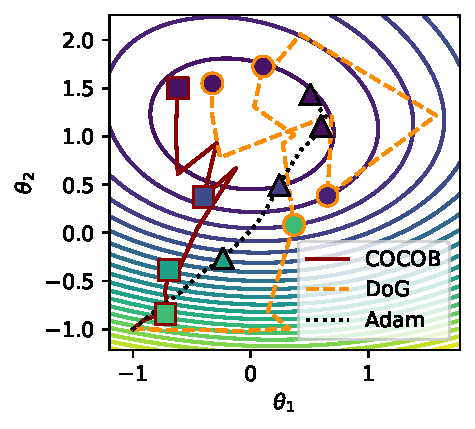
\includegraphics[width=0.4\textwidth]{figures/sgd_trajectory_optims1.pdf}};

		% Lower image
		\node[inner sep=0pt, below=3mm of upper] (lower){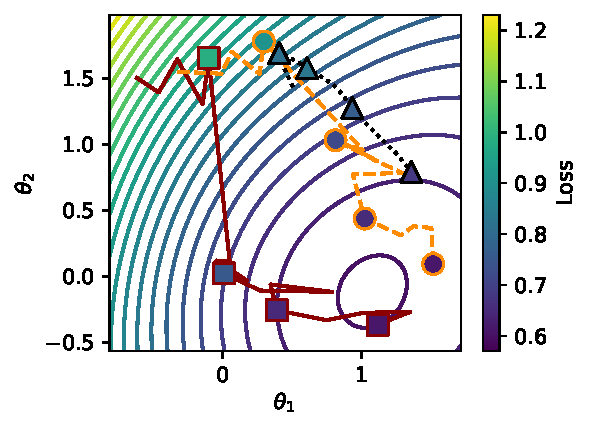
\includegraphics[width=0.4\textwidth]{figures/sgd_trajectory_optims2.pdf}};

		\path ([xshift=-8pt]upper) -- ([xshift=-8pt]lower) node[midway] (text){Concept Drift};
		\draw[->] ([xshift=-5pt, yshift=5pt]upper.south-|text.west) -- ([xshift=-5pt, yshift=-3pt]lower.north-|text.west);
		\draw[->] ([xshift=5pt, yshift=5pt]upper.south-|text.east) -- ([xshift=5pt, yshift=-3pt]lower.north-|text.east);

	\end{tikzpicture}
	\caption{Parameter trajectory of COCOB~\cite{orabonaTrainingDeepNetworks2017}, DoG~\cite{ivgiDoGSGDBest2023} and Adam~\cite{kingmaAdamMethodStochastic2017b} on synthetic data stream with abrupt concept drift. Marker colors depict the expected prequential loss over the last 16 data instances.}
\end{figure}

\section{Conclusion}


\bibliography{aaai24}

\end{document}
